\documentclass[a4paper,10pt]{article}

\usepackage{graphicx}
\usepackage{fancyhdr}
\usepackage{geometry}
\usepackage{amsmath}
\usepackage{blindtext}
\usepackage{rotating}
\usepackage{wrapfig}

% Page Geometry
\geometry{a4paper, total={170mm,257mm}, left=20mm, right= 20mm, top=30mm, bottom = 30mm, headheight=40pt}

% Page Header/Footer Setup
\pagestyle{fancy}
\fancyhf{}
\lhead{\includegraphics[width=2cm]{IIITB_Logo.jpg}} 
\lfoot{International Institute of Information Technology, Bangalore}
\rfoot{Page \thepage}

% Title Details
\title{\Large\textbf{2 - Bit Calculator and 3 - Bit Timer} \\
    \normalsize Course Name: ESS 102, Digital Design \\ % Replace XXXXXX with Course Code

    \normalsize Students Name: Shubhranil Basak(510), Gathik Jindal(089), Ahilnandan Kabilan(614), Archit Jaju(128) \\ % Replace XXXXXXX with Student Name
    \normalsize Student ID: IMT2023510, IMT2023089, IMT2023614, IMT2023129\\ % Replace XXXXXXX with Student ID    
    \normalsize Group ID: 40 \\%
    }
\date{30 November 2023} % displays the date. Leave it blank, if you don't want to display the date.

\begin{document}

\maketitle
\thispagestyle{fancy} 

\section{Combinational Circuit: 2-bit Calculator}

\subsection{Introduction}
This project report explores the details of digital electronics, uncovering how combinational. We focus on combinational circuits with the careful building of a 2-bit calculator. This calculator smoothly combines different electronic parts, doing basic math like adding, subtracting, multiplying, and dividing. The stated operations are selected by using a multiplexer which has two select lines. The report goes through the basic ideas, design details, and how well the calculator performs. In this exploration, the project report breaks down the technical parts of combinational.

\subsection{Description}
The 2-bit Calculator is a unique calculator that operates on two bits of binary information. This calculator allows users to perform basic arithmetic operations on two 2-bit binary numbers. It provides a simple and intuitive interface for inputting and calculating binary values. The operator is selected by using two select lines for addition, subtraction, multiplication and division. The numbers are inputted in binary format. We have also tried to include a method to display our output using a 7-segment display decoder.

The key components required were:\newline
    1. 2 bit Adder circuit to implement addition.\newline
    2. 2 bit Subtractor circuit to implement subtraction.\newline
    3. 2 bit Multiplier circuit to implement multiplication.\newline
    4. 2 bit Divider circuit to implement division.\newline
    5. 7 - Segment Display Decoder to display our output appropriately.\newline

\subsection{Working}

\subsubsection{Adders}
Adder’s are really simple to implement in digital design using combinational logic. We use half adders to make a full adder. Mostly one bit adders are used repeatedly to make multiple bit adders. This type of design is called a ripple adder due to how the circuit is designed and simulated. Using a look ahead adder is obviously more efficient since it saves a lot of time. But using it in a project as big as ours does not really make sense and hence we went along with the normal simple logic of using a simple adder. Writing the Boolean equations is a really easy task, hence we leave it as a fun in-project exercise for the reader to solve :P.
\subsubsection{Subtractor}
The subtractor circuit used in the project is a simple digital logic circuit with two output bits and four input bits. The Boolean equations for the subtractor were calculated using Karnaugh maps (K-maps) and a truth table. The truth table was relatively straightforward, with the difference between two binary numbers as the output in a two-bit number. The K-maps were then simplified to obtain the Boolean equations for the subtractor, which were then used to create the subtractor subcircuit in LTspice. The subtractor subcircuit is implemented using simple logic gates, such as AND, OR, and NOT gates.\newline\newline
Boolean Equations:\newline
\hspace*{2cm} \[a = b_3 + b_1 + (b_0 \odot b_2) \hspace*{1cm}  b = (b_0 \odot b_1) + b_3 + \overline{b_2}\]\newline
\hspace*{2cm} \[c = b_0 + \overline{b_1} + b_2 + b_3 \hspace*{1cm}  d = \overline{b_0}(b_1 + \overline{b_2}) + b_0 \overline{b_1} b_2 + b_3 + b_1 \overline{b_2}\]\newline

\subsubsection{Multiplier}
This multiplier subcircuit used in the project is designed to multiply two 2-bit binary inputs, and represent it using a 4-bit output. The expressions for b3 and b2 is obtained utilizing the K map taking values from the truth table. For b1 and b0 it utilized multiplexers. Despite the drawback of not always being an optimized solution, I found that the usage of multiplexers makes it convenient to implement, debug, and understand. The circuit has a very limited number of gates so the inefficiency doesn’t count much.\newline\newline
Boolean Equations:\newline 


\subsubsection{Divider}
The divider we have used in our project is a very simple circuit. It’s directly made from mapping each input to its output. It was made possible by making a simple truth table and then mapping each input and output in a k-map. Then this K-map was simplified and the circuit was made using the simplified Boolean expressions obtained from the k - map. It involves the usage of and or and not gates. I attached a picture of the symbol on the side for better understanding.\newline\newline
Boolean Equations:\newline 
\hspace*{4.5cm}\[ y_0 = \overline{a_1}a_0b_0 + b_1b_0(a_0 + a_1) + a_1\overline{a_0}b_1 \]
\hspace*{4.5cm}\[ y_1 = a_0b_1(b_0 + \overline{a_1}) \]

\subsubsection{7 Segment Display Decoder}
The 7-segment display decoder used in our is a simple circuit. It was made by first converting the binary input to decimal and deciding which segment(a, b, c, d, e, f, g) would need to light up to display the desired number. Then a K-map was made for each segment of the decoder and was simplified to a simple Boolean expression. Then these expressions were used to design the logic for every segment from A-G. The gates used in making this 7-segment display decoder are AND, NOT, XOR, NOR, and OR gates. \newline\newline
Boolean Equations:\newline
\hspace*{2cm} \[a = b_3 + b_1 + (b_0 \odot b_2) \hspace*{1cm}  b = (b_0 \odot b_1) + b_3 + \overline{b_2}\]\newline
\hspace*{2cm} \[c = b_0 + \overline{b_1} + b_2 + b_3 \hspace*{1cm}  d = \overline{b_0}(b_1 + \overline{b_2}) + b_0 \overline{b_1} b_2 + b_3 + b_1 \overline{b_2}\]\newline

\subsection{Results}
Obviously, describing the test-cases here would take up a lot of space, so please do try running the simulation on your computer and see it for yourself. The test bench provided for the calculator can be tested in LT-Spice.\newline\newline
The following are the select lines encoding for the different operations that our simulation solves for:\newline\newline
0 0 - Division,\newline
0 1 - Addition,\newline
1 0 - Multiplication,\newline
1 1 - Subtraction.
\newline\newline
\section{Sequential Circuit: 3-Bit Timer}

\subsection{Description}
Its a simple mealy FSM (Finite state Machine) that implements a timer. It outputs 0 until the elapsed time is equal to the time set by the user, and then it outputs 1 for the rest of time. Obviously this can be altered using an external asynchronous reset. This uses a 3 bit up counter or a mod 8 counter and a 3 bit magnitude comparator to function. Since FSMs take a long time to implement to in LT Spice, this is implemented in python and the we have used matplotlib library to plot all our inputs and outputs and various other states that we would like to monitor.

\subsection{Implementation}
The device works, using a mod 8 up counter with an enable input and a 3 bit magnitude comparator. The mod 8 counter first keep counting until enable is 0, and when it is so it stops counting and remains in the same position indefinitely. The magnitude comparator checks if the output of the counter. The only output of our comparator is if the two binary numbers are equal and if it is so it goes as $\boldsymbol{\overline{en}}$, enabling and disabling the counter. The inputs are supposed to be given by the user in the start itself, hence we have defined our intput in the start of the python program, in the class $\boldsymbol{MooreMachine}$ iteself. Our $\boldsymbol{input_schedule}$ list is empty because we don't expect the user to change their input value while the timer is running.

\subsection{Boolean equations for next state logic}
Here $\boldsymbol{y_0}$, $\boldsymbol{y_1}$, $\boldsymbol{y_2}$ are the next state and $\boldsymbol{q_0}$, $\boldsymbol{q_1}$, $\boldsymbol{q_2}$ are the present state bits and $\boldsymbol{en}$ is the enable bit.\newline
\[y_0 = q_0\overline{en} + \overline{q_0}en\]
\[y_1 = \overline{en}q_1 + q_1\overline{q_0} + en\overline{q_1}q_0\]
\[y_2 = \overline{en}q_2 + q_2\overline{q_1} + q_2\overline{q_0} + en\overline{q_2}q_1q_0\]

\subsection{Wave Forms}
Here, to make it easier to visualise I have changed the input everytime the timer finishes counting upto the desired time (which is inputted by the user). Here I have tested for every possible time from 7 to 1, counting to zero obvisouly doesn't make sense. Here if you carefully notice you will notice that there is a very small error in the time. But that can be easily fixed by taking a much faster clock speed. The faster the clock frequency the more precise will our timer be.\newline
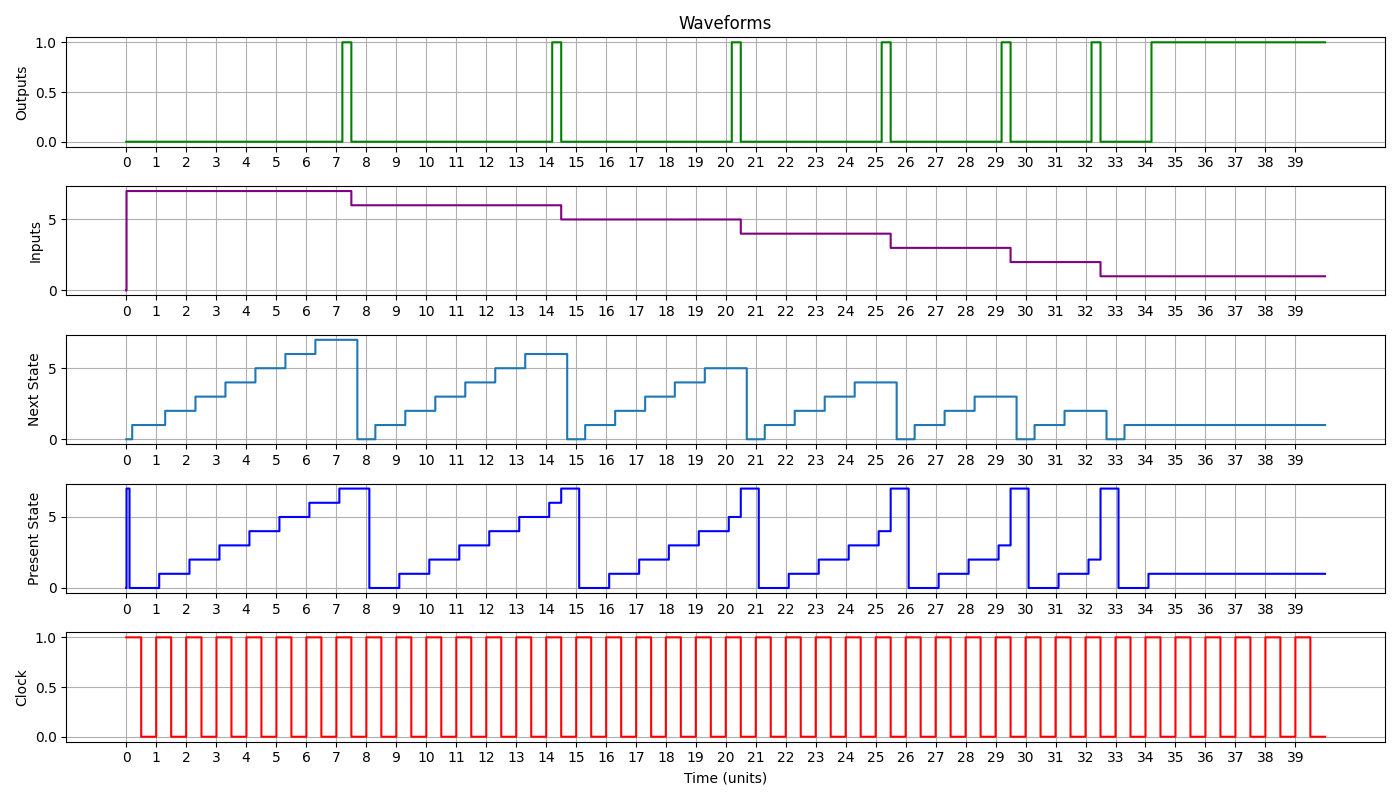
\includegraphics[scale=0.5]{wave_form.png}

\subsection{State Transition Diagram}
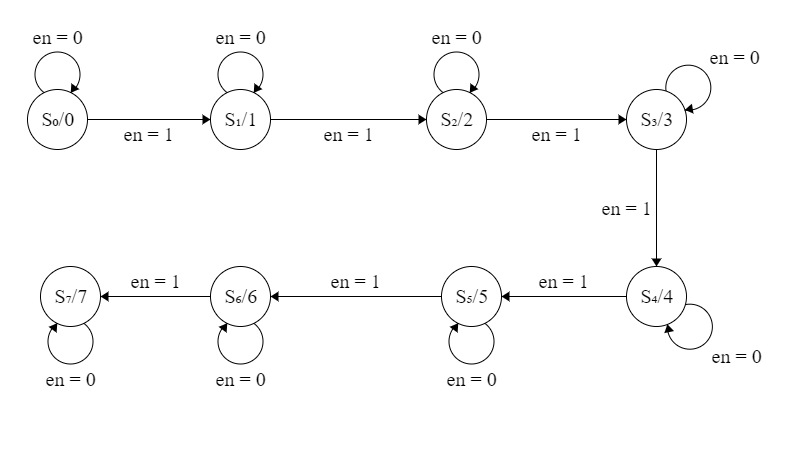
\includegraphics[scale=0.75]{state_dia.png}

\subsection{Results}
The timer works perfectly, it takes in input in the MooreMachine class defined in main.py. The counter stops counting when it has counted exactly to what it was required to count up to. Obviously an asynchronous reset can be incorporated in the design and hence the timer can be used multiple times. There are many other implementations for the same circuit. We could use multiple ways to make our counter, our magnitude comparator, and obviously our fsm too.


% \bibliographystyle{IEEEtran}
% \bibliography{refs} 
\end{document}
